\section{Введение}
Пусть имеется действительная на интервале $\left[-\pi \leqslant t \leqslant \pi \right]$, конченая и непрерывная функция $f(t)$. Тогда на этом интервале ее можно представить в виде ряда Фурье:
\begin{equation}
    f(t) = A_0 + \sum \limits_{k = 1}^{\infty}\left[A_k \cos{kt} + B-k \sin{kt} \right]
    \label{Fourier_series}
\end{equation}
Коэффициенты ряда можно найти по формулам:
\begin{align}
    A_0 & {} = \frac1{2\pi}\int \limits^{\pi}_{-\pi}f(t)\,dt \\
    A_k & {} = \frac1{\pi} \int \limits^{\pi}_{-\pi}f(t) \cos{kt}\, dt \\
    B_k & {} = \frac1{\pi} \int \limits^{\pi}_{-\pi}f(t) \sin{kt}\, dt
    \label{Fourier coofitients}
\end{align}

Откуда же берутся эти формулы?

В данном случае функции $\varphi_k(t) = \sin{kt}$ и $\psi_k(t) = \cos{kt}$ и $\varphi_0(t) = 1$ для любых целых неотрицательных $k$ это базис, на котором строится целевая функция $f(t)$. Для таких функций определено скалярное произведение:
\begin{equation}
    \langle g(t) \text{,} h(t) \rangle = \int \limits^{\pi}_{-\pi} g(t)h(t)\, dt
\end{equation}
Причем:
\begin{align*}
    \langle \varphi_k, \varphi_m \rangle & {} = 0 & k \neq m \\
    \langle \psi_k, \psi_m \rangle & {} = 0 & k \neq m\\
    \langle \psi_k, \varphi_m \rangle & {} = 0 &  \forall k, m \in\mathbbm{N} \cup 0
\end{align*}
Однако при этом:
\begin{equation}
    \langle \varphi_k, \varphi_k \rangle = \langle \psi_k, \psi_k \rangle = \pi \qquad \forall k \in\mathbbm{N} \cup 0\\
\end{equation}
Отсюда, если мы скалярно умножим формулу (\ref{Fourier_series}) по обе стороны знака равенства на $\varphi_k(t)$, $\psi_k(t)$ и $\varphi_0$, то получим формулы (\ref{Fourier coofitients}).
    
    Зная, что гармонические функции $\sin{x}$ и $\cos{x}$ представимы через формулы Эйлера:
\begin{equation}
    \sin{x} = \frac{e^{ix} - e^{-ix}}{2i}\qquad   \cos{x} = \frac{e^{ix} + e^{-ix}}{2}
\end{equation}
Поэтому можем представить ряд Фурье в обобщенном виде:
\begin{equation}
    f(t) = \sum \limits^{+\infty}_{k = -\infty} C_k e^{-ikt}
\end{equation}
Где:
\begin{equation}
    C_k = \frac1{2\pi}\int \limits_{-\pi}^{\pi}f(t)e^{-ikt}\,dt
    \label{ob_ck}
\end{equation}
Связь между (\ref{Fourier coofitients}) и (\ref{ob_ck}) выражается формулами:
\begin{equation*}
    C_k=A_k - iB_k \qquad C_{-k}= A_k + iB_k
\end{equation*}

Однако разложение можно обобщить еще дальше, а именно представить, что частоты $k$ изменяются не дискретно, а непрерывны. В таком виде интегралы:
\begin{align}
    f(t) & {} = \int \limits^{+\infty}_{-\infty}F(\omega)e^{2\pi i \omega t}\, d\omega\\
    F(\omega) & {}= \int \limits^{+\infty}_{-\infty}f(\tau)e^{-2\pi i \omega \tau}\, d\tau
    \label{fourier_transform}
\end{align}
называются взаимообратными трансформантами Фурье.

Вообще в реальном мире сигнал с детектора (импульс), можно представить в виде гистограммы. На самом деле так и происходит, ведь мы не можем записать аналоговый сигнал в файл, однако можем записывать значение напряжения или тока через малые промежутки времени, как это делают цифровые осциллографы и диджитайзеры. Так что по факту, когда мы получаем данные для обработки, он всегда является гистограммой, а для них применяется другое - дискретное преобразование Фурье.

Дискретное преобразование Фурье в качестве базиса имеет функции на строго определенных частотах, определяемых исключительно количеством проведенных за период измерений сигнала.
Формула дискретного преобразования Фурье выглядит следующим образом:
\begin{equation}
    \mathrm{X}(j) = \sum \limits_{k = 0}^{N-1}A_k\exp{-\frac{2\pi i }{N}jk}
\end{equation}
Здесь $j$ - дискретное время. $j = 0\text{, }1\text{,}\ldots\text{,}N-1$.
$k$ - индекс дискретной частоты. $k = 0\text{, }1\text{,}\ldots\text{,}N-1$. Сама дискретная частота определяется формулой $\frac{k}{T}$, где $T$ - период в течении которого проводились измерения. $A_k$ - комплексные коэффициенты, фактически комплексные амплитуды сигналов, то есть хранящие информацию и об амплитуде и о фазе сигнала. $N$ - количество измеренных точек (сэмплов). Для расчета Фурье-образа или оригинала требуется $N^2$ операций комплексного сложения и умножения, однако если выкинуть члены ряда, значения которых мы значем, то вычисления будут проходить быстрее. На основе этого факта Кули и Тьюки придумали алгоритм быстрого преобразования Фурье. Пусть массив, на который мы накладываем преобразование Фурье имеет размер $N = 2^m$. Тогда выражение $N\log_2 N = mN$ будет характеризовать время выполнения расчетов. Например при $m =13$ необходимо выполнить около 8 тыс. операций. Обычное Фурье преобразование справится с таким массивом за полчаса, а быстрое всего за 5 миллисекунд. 
\begin{figure}
    \centering
    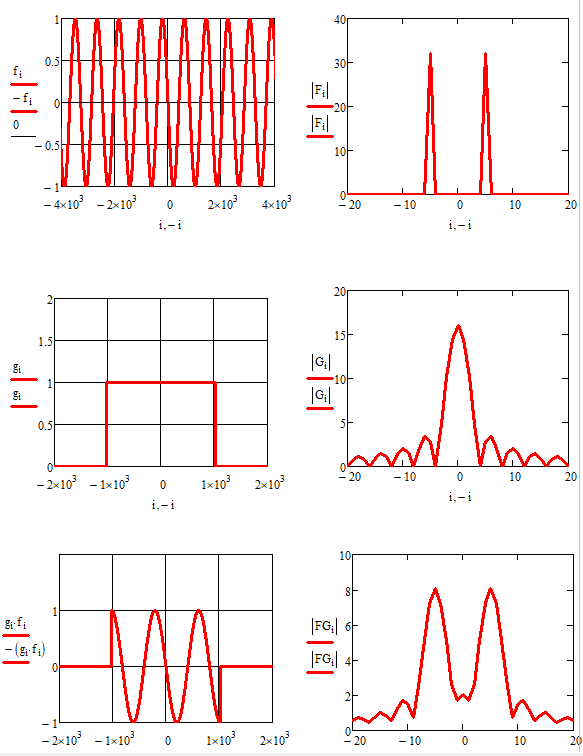
\includegraphics[scale = 0.8]{Pictures/Fourier.png}
    \caption{\centering Преобразование Фурье для функций (сверху вниз):
             1. $\sin{\left(10\pi t\right)}\quad t \in [-5\pi; 5\pi]$.
             2. Ступенька с амплитудой $1 \quad t \in [-\pi; \pi]$.
             3. Произведение функций 1 и 2.}
    \label{fig:fourier_example}
\end{figure}
Для того, чтобы понимать как работает Фурье преобразование рассмотрим графики на рис. \ref{fig:fourier_example}. Данные рисунки получены в маткаде. Качество их оставляет желать лучшего, однако автору показалось, что данный инструмент хоть и с некоторыми ограничениями, но довольно наглядно представляет предмет разговора. Читателю не стоит обращать внимание на подписи левых осей абсцисс данных графиков, поскольку они лишь симулируют используя инструмент быстрого преобразования Фурье, как работало бы настоящее преобразование Фурье для показанных функций. Далее детально разберем представленный рисунок. В левом верхнем углу изображен график функции $\sin{(10\pi t)}$, то есть обычная синусоида с частотой 5. При взятии ее образа Фурье по формулам (\ref{fourier_transform}) мы получим две $\delta$-линии расположенные симметрично относительно нуля на расстоянии соответствующему $i=\pm5$, то есть частоте 5. Важно понимать, что если бы частота равнялась $\nu$, то и $\delta$-линии располагались бы симметрично относительно нуля на расстоянии  $i=\pm \nu$. То есть преобразование Фурье показывает какие частоты содержатся в данной функции. Можно также провести соответствие с тем, что разложение обычной синусоиды в ряд Фурье, что очевидно, равно само себе.

Следующая функция, изображенная на рисунке - ступенька. Ее Фурье образ выглядит, как показано правее. Форма этой кривой описывается так называемой функцией Уиттикера - $\frac{\sin{x}}{x}$ (правда функция Уиттикера, вообще говоря, дискретна, однако форма частотной кривой имеет именно такое аналитическое выражение). \textbf{Положения, где частотная кривая пересекает абсциссу обратно пропорциональны длине импульса.} То есть, если бы наша ступенька была длиннее, то пик был бы уже.

Третья картинка показывает Фурье преобразование для произведения предыдущих функций и тут, на самом деле, чисто интуитивно ясно, что так оно и должно быть, однако все же стоит сказать о свертке.

Для этого рассмотрим задачу из теории вероятности: \textit{Пусть есть две случайные величины $x$ и $y$ с известными законами распределения $\rho_x(x)$ и $\rho_y(y)$. Необходимо найти распределение $\rho_z(z)$ для случайной величины $z=x+y$.}

Так как величины $x$ и $y$ независимы, то вполне очевидно, что в случае, если бы величны принимали только конкретные значения $\rho_z = \rho_x\rho_y$. То есть вероятность какого-то конкретного $z$ есть произведение вероятностей что $x$ и $y$ будут в сумме давать $z$. Но необходимо найти именно функцию $\rho_z(z)$, поэтому можем записать так:
\begin{equation*}
    \rho_x(x)\rho_y(y) = \rho_x(x)\rho_y(z -x)
\end{equation*}

Если мы проинтегрируем это выражение по $x$, то получим искомую функцию, так как фактически мы просуммируем все вероятности значений $x$ и $y$, при котором $x+y=z$:
\begin{equation*}
    \rho_z(z) = \int \rho_x(x)\rho_y(z -x)\, dx 
\end{equation*}

Интеграл такого типа называется интегралом типа свертки. Если бы мы варажали вместо $x$ величину $y$, то результат был бы тот же, что тоже, в принципе, понятно.

Одно из свойств Фурье преобразования, которое как раз используется в третьем преобразовании на рис. \ref{fig:fourier_example} как раз использует свертку:
\begin{equation}
    h(t)g(t) \xrightarrow{\mathscr{F}}H(\omega) * G(\omega)
    \label{svertka}
\end{equation}

Звездочка в выражении (\ref{svertka}) как раз обозначает свертку. То есть Фурье преобразование произведения функций есть свертка изображений этих функций.

Предыдущему примеру с распределениями вероятностей можно сопоставить простой физический пример: $x$ это может быть полезный сигнал с детектора, а $y$ шумовой сигнал. Их сумма дает величину на выходе, равную $z$.

Рассмотрим другой пример с использованием свертки. Пусть регистрируем излучение с двумя равновероятными энергетическими модами. То есть ожидаем получить спектр вида рис \ref{fig:f(x)}. Эта функция представляет собой сумму двух гауссовских пиков со средними 20 и 30 соответственно и дисперсией 10. Пусть функция отклика детектора представляет также гауссовский колокол (рис. \ref{fig:primer} a). Результирующий спектр представлен на рисунке (рис. \ref{fig:primer} б). Как видно, при малых дисперсиях функции отклика, ее форма, отличная от дельта линии слабо влияет на форму спектра, однако при значениях дисперсии соразмерных и более, чем у пиков в реальном спектре, наблюдаемый спектр будет уширяться вплоть до того, что моды будут не различимы.
\begin{figure}
    \centering
    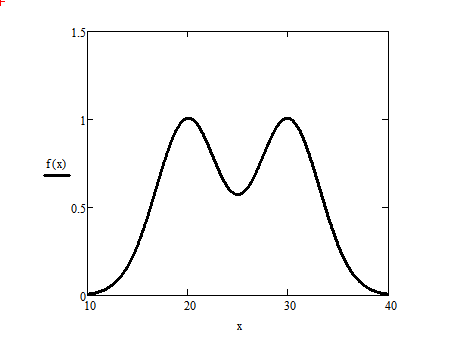
\includegraphics{Pictures/f(x).png}
    \caption{Пример измеряемого спектра.}
    \label{fig:f(x)}
\end{figure}
\begin{figure}[h]
\begin{minipage}[h]{0.49\linewidth}
\center{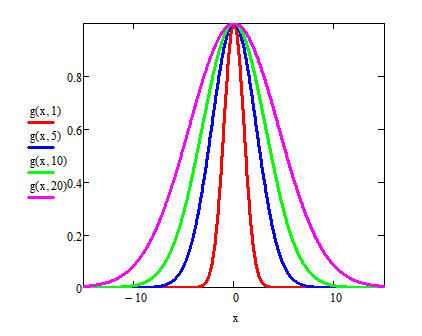
\includegraphics[scale = 0.65]{Pictures/g(x).png} \\ (а)}
\end{minipage}
\hfill
\begin{minipage}[h]{0.49\linewidth}
\center{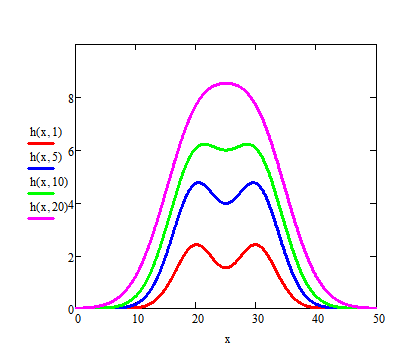
\includegraphics[scale = 0.65]{Pictures/h(x).png} \\ (б)}
\end{minipage}
\caption{Функция отклика детектора (а). Спектр на выходе детектора (б)}
\label{fig:primer}
\end{figure}

Мы уже убедились в том, что с помощью ряда Фурье можно разложить любые функции на гармонические составляющие, то есть на сумму синусов и косинусов с различными частотами. Однако в реальной жизни мы не можем раскладывать функцию в бесконечный ряд, поэтому мы вынуждены сталкиваться с некоторыми вполне закономерными ограничениями. Очевидно, что на разложение прямоугольного импульса (как на рис. \ref{fig:fourier_example} левый средний) требуется больше членов ряда, чем, например для функции отклика детектора из предыдущего примера, поскольку у первого более крутые фронты, а значит максимальная частота в его спектре разложения стремится к бесконечности, чего по факту быть не может. Поэтому все полосы пропускания различных электрических приборов и имеют гаусоподобную форму с плато вместо пика. В случае, если, все-таки, прямоугольный импульс проходит через некоторый кабель с небесконечной полосой пропускания, то в конечном итоге увидим завал фронтов нашего импульса.

Часто возникает необходимость в определении частотного состава сигнала. Это наиболее важно, когда та или иная частота несет в себе какую-либо информации через сигнал. Простой пример: наводки на детекторе. Нередко бывает так, что из-за плохого контакта с сетью, на выходе детектора сигналы выглядят не совсем так, как мы ожидаем. Можно сказать, что они выглядят "неровно". В этом случае Фурье преобразование может помочь нам определить, действительно ли дело в наводках, или нет. Об этом нам как раз скажет пик на частоте порядка $50$ Гц. 

Если в результирующем сигнале присутствуют близкие частоты, то возможность их разделения зависит от времени измерения сигнала или, как еще говоря <<временные ворота>>, то есть промежуток времени, за который мы сэмплируем сигнал. На рис. \ref{fig:rect_05} показан сигнал из трех частот 5, 20, 21 Гц соответственно, а также его Фурье спектр после измерения в течении $0.5$ секунд. 

\begin{figure}[!h]
    \centering
    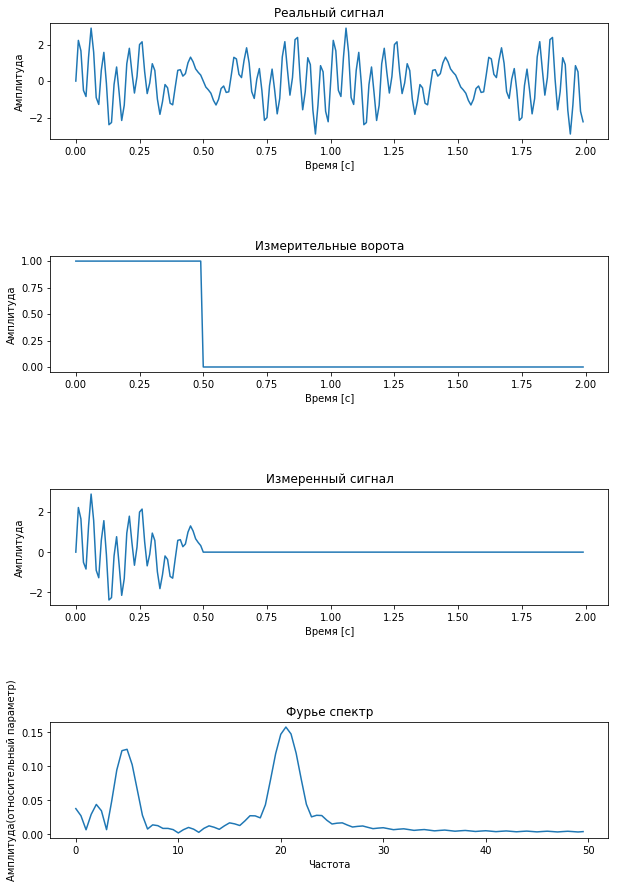
\includegraphics[scale = 0.5]{Pictures/no_separation_rectangular.png}
    \caption{Измерение сигнала и его Фурье спектр при времени измерения $0.5$ c.}
    \label{fig:rect_05}
\end{figure}

Как видим, при такой длительности измерения частоты две последние частоты не разделяются и на спектре Фурье мы видим всего один пик. Давайте посмотрим, что будет, если увеличить время измерения в два раза (рис.\ref{fig:rect_1})

\begin{figure}[!h]
    \centering
    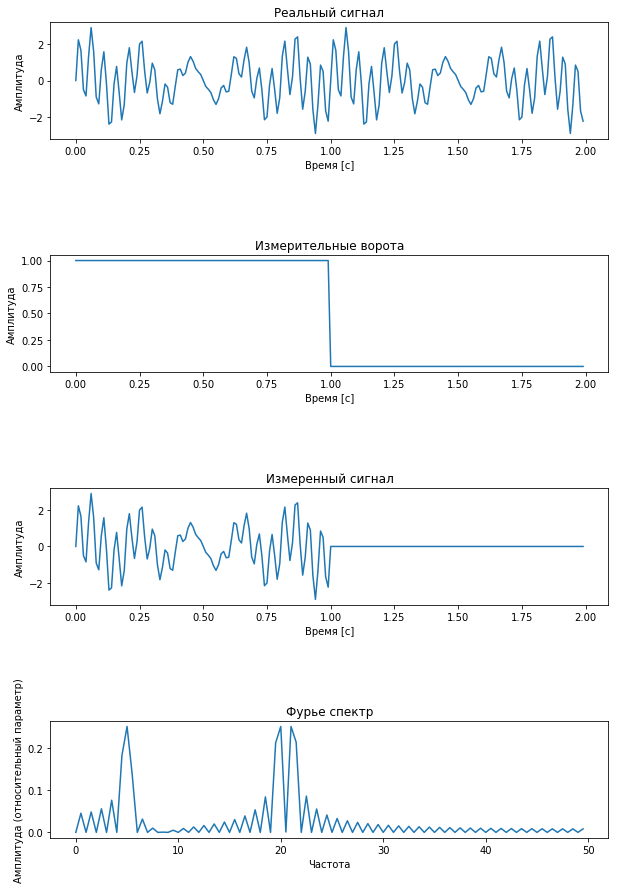
\includegraphics[scale = 0.5]{Pictures/separation_rectangular.png}
    \caption{Измерение сигнала и его Фурье спектр при времени измерения $1$ c.}
    \label{fig:rect_1}
\end{figure}

В этом случае стало хорошо видно наличие двух разделенных частот. 

Это, возможно, трудно представить, но возможны и другие формы временных окон, то есть не обязательно прямоугольные. Однако в случае с прямоугольным окном разделение частот проще, поскольку в его разложении в ряд Фурье, можно сказать, находятся все частоты, от самых малых, до бесконечно больших. Если окно, например, треугольной или гаусоподобной формы, то для разделения частот необходимо большее время измерений, поскольку фронты таких окон менее крутые, а следовательно содержат в себе более низкие частоты.

В общем и целом для различия частот необходимо выполнение следующего условия:
\begin{equation}
    T\geqslant \frac{1}{f_1 - f_2}
\end{equation}
где $T$ - ширина временного окна, а $f_1$ и $f_2$ - частоты, которые мы хотим разделить.